\newpage
\section{Methods}\label{sec:methods}

This section describes the design and implementation of a guided consultation assistant for dementia care communications, addressing the identified gap between general-purpose clinical decision support systems and the specific communication needs of primary care providers conducting dementia consultations.

% ============================================================
\subsection{System Design and Development}\label{sec:system_design}

This project employed a design and development methodology to create a guided consultation assistant for dementia care in primary care settings. The approach combined structured communication frameworks with large language model capabilities through retrieval-augmented generation.

The system was designed according to three guiding principles derived from identified gaps in existing clinical support tools (Section~\ref{sec:relatedwork}):

\begin{enumerate}
    \item \textbf{Communication-centeredness}: Unlike documentation-focused AI systems, the proposed tool actively guides clinicians through consultation phases and relational communication challenges.
    \item \textbf{Domain specificity}: Rather than general clinical decision support, the system provides evidence-based communication strategies tailored to dementia consultations.
    \item \textbf{Source fidelity}: All guidance is grounded in explicit citations from validated resources, avoiding hallucinations and unsupported claims.
\end{enumerate}

The development process followed an iterative design approach, progressively incorporating:
the Navigation Map framework for consultation structure,
the Stuck Points Framework for relational communication support,
and the Conversation Guides for sample language.


% ============================================================
\subsection{Framework Architecture}\label{sec:framework}

The system integrated three interconnected components from the Ariadne Labs Essential Communications Toolkit: the Navigation Map, the Conversation Guides, and the Stuck Points Framework.

\subsubsection{Navigation Map}

The Navigation Map provided the overarching consultation structure, organizing the dementia care journey into three sequential phases:

\begin{enumerate}
    \item \textbf{Recognition}: Initial identification of cognitive concerns through patient, family, or clinician observation.
    \item \textbf{Evaluation}: Systematic assessment including functional evaluation, cognitive testing, medication review, and targeted examination.
    \item \textbf{Diagnosis}: Sharing findings, applying diagnostic impressions, and planning follow-up care.
\end{enumerate}

Each phase included defined entry and exit criteria, enabling the system to track consultation progress and suggest appropriate next steps.

\subsubsection{Conversation Guides}

The Conversation Guides provided ready-to-use language and dialogue strategies tailored to each phase of the Navigation Map. These guides were designed to ensure honesty, compassion, and clarity during sensitive conversations. Sample language addressed common scenarios including:

\begin{itemize}
    \item Introducing cognitive assessment to patients and families
    \item Assessing function across daily living activities
    \item Conducting cognitive screening (e.g., Mini-Cog)
    \item Communicating normal versus concerning findings
    \item Delivering diagnostic impressions (MCI, dementia)
    \item Addressing emotional responses and questions
\end{itemize}

The guides emphasized patient-centered communication principles including:
acknowledging uncertainty, centering the patient's story, addressing emotions, and reframing success from diagnosis to explanation and care optimization.

\subsubsection{Stuck Points Framework}

The Stuck Points Framework addressed relational communication obstacles that arise during sensitive clinical conversations. It provided a structured approach to identifying and resolving moments where communication became difficult or stalled:

\begin{enumerate}
    \item \textbf{Notice and Reframe}: Recognizing tension and viewing it as an opportunity for trust-building
    \item \textbf{Pause and Name It}: Acknowledging the stuck point and asking permission to explore
    \item \textbf{Acknowledge Emotion}: Addressing emotional experiences before problem-solving
    \item \textbf{Get Curious and Explore}: Understanding underlying reasons through open questioning
    \item \textbf{Summarize and Plan}: Recapping and establishing next steps with reassurance
\end{enumerate}

The framework included suggested language for each step, enabling clinicians to navigate relational challenges while maintaining therapeutic alliance.



% ============================================================
\subsection{Knowledge Base Construction}\label{sec:knowledge_base}

The knowledge base was constructed by structuring and indexing content from the Ariadne Labs Essential Communications Toolkit. The construction pipeline comprised three main stages:

\begin{enumerate}
    \item \textbf{Source material organization}: The toolkit documents were parsed and separated into three thematic components: the Navigation Map structure, the Conversation Guides with sample language, and the Stuck Points Framework.
    \item \textbf{Chunking strategy}: Each component was divided into semantically coherent chunks, preserving the hierarchical structure (phase $\rightarrow$ subsection $\rightarrow$ specific guidance).
    \item \textbf{Embedding and indexing}: Each chunk was converted to a vector embedding and stored in a searchable index for retrieval-augmented generation.
\end{enumerate}

The knowledge base construction is summarized in Figure~\ref{fig:preprocessing_pipeline}.

% =====================FIGURE START============================

\begin{figure}[p]
\centering
% --- Knowledge base construction pipeline (TikZ) ---
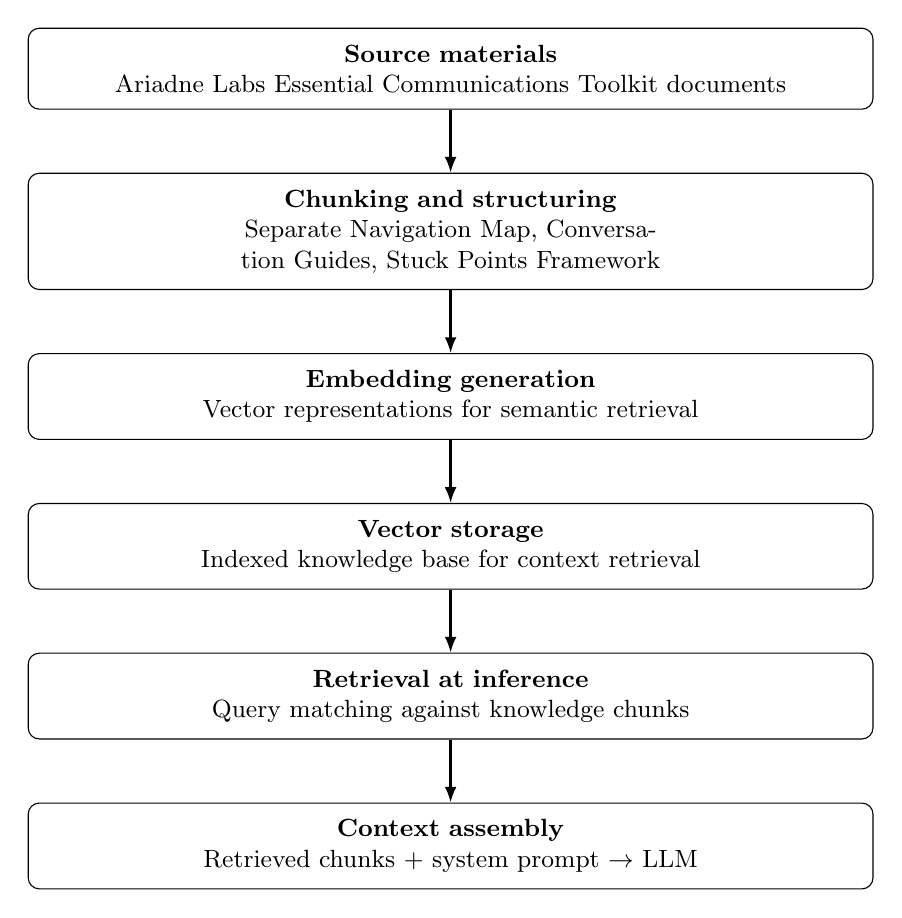
\begin{tikzpicture}[
  font=\small,
  node distance=8mm,
  box/.style={draw, rounded corners, align=center, inner sep=6pt, text width=0.85\textwidth},
  arrow/.style={-{Latex[length=2mm]}, thick}
]
\node[box] (source) {
\textbf{Source materials} \\
Ariadne Labs Essential Communications Toolkit documents
};
\node[box, below=of source] (parse) {
\textbf{Chunking and structuring} \\
Separate Navigation Map, Conversation Guides, Stuck Points Framework
};
\node[box, below=of parse] (embed) {
\textbf{Embedding generation} \\
Vector representations for semantic retrieval
};
\node[box, below=of embed] (store) {
\textbf{Vector storage} \\
Indexed knowledge base for context retrieval
};
\node[box, below=of store] (retrieve) {
\textbf{Retrieval at inference} \\
Query matching against knowledge chunks
};
\node[box, below=of retrieve] (context) {
\textbf{Context assembly} \\
Retrieved chunks + system prompt $\rightarrow$ LLM
};
\draw[arrow] (source) -- (parse);
\draw[arrow] (parse) -- (embed);
\draw[arrow] (embed) -- (store);
\draw[arrow] (store) -- (retrieve);
\draw[arrow] (retrieve) -- (context);
\end{tikzpicture}
\caption{
Knowledge base construction and retrieval pipeline.
The system used retrieval-augmented generation to ground responses in validated toolkit resources.}
\label{fig:preprocessing_pipeline}
\end{figure}


% =====================FIGURE END==============================

\subsection{LLM System Implementation}\label{sec:llm_implementation}

The consultation assistant employed a retrieval-augmented generation architecture that combined clinician queries with relevant toolkit context.

\subsubsection{Application architecture}

The consultation assistant was implemented as a web application using modern frontend technologies to enable rapid prototyping and clinician accessibility:

\begin{itemize}
    \item \textbf{Next.js}: React framework providing server-side rendering, routing, and API routes for LLM integration
    \item \textbf{TailwindCSS}: Utility-first CSS framework for responsive, consistent UI styling
    \item \textbf{Firebase}: Backend-as-a-service platform providing authentication, real-time database, and cloud functions for secure API key management
    \item \textbf{Harvard Canvas API}: Integration with institutional learning management system for potential future deployment in educational contexts
\end{itemize}

The application architecture followed a client-server model where the frontend handled clinician input, context display, and response rendering, while LLM inference was performed server-side through API routes to protect API credentials. Firebase authentication enabled role-based access control for potential multi-clinician deployment scenarios.

\subsubsection{Input processing}

Clinician queries were processed to extract semantic meaning and determine the consultation context. The system used a structured prompt template that specified:
\begin{itemize}
    \item The clinician's role and the system's purpose
    \item The three-phase consultation framework (Recognition, Evaluation, Diagnosis)
    \item Grounding rules requiring responses to cite toolkit sources
    \item Output format specifications including section headers
\end{itemize}

\subsubsection{Retrieval-augmented generation}

At inference time, the system retrieved relevant knowledge chunks based on the clinician's query. These chunks were assembled into the prompt context, enabling the LLM to generate responses grounded in validated toolkit resources. The retrieval mechanism used semantic similarity matching against the indexed knowledge base.

The architecture is summarized in Figure~\ref{fig:model_architecture}.

% =====================FIGURE START============================

\usetikzlibrary{positioning,arrows.meta}

\begin{figure}[p]
\centering
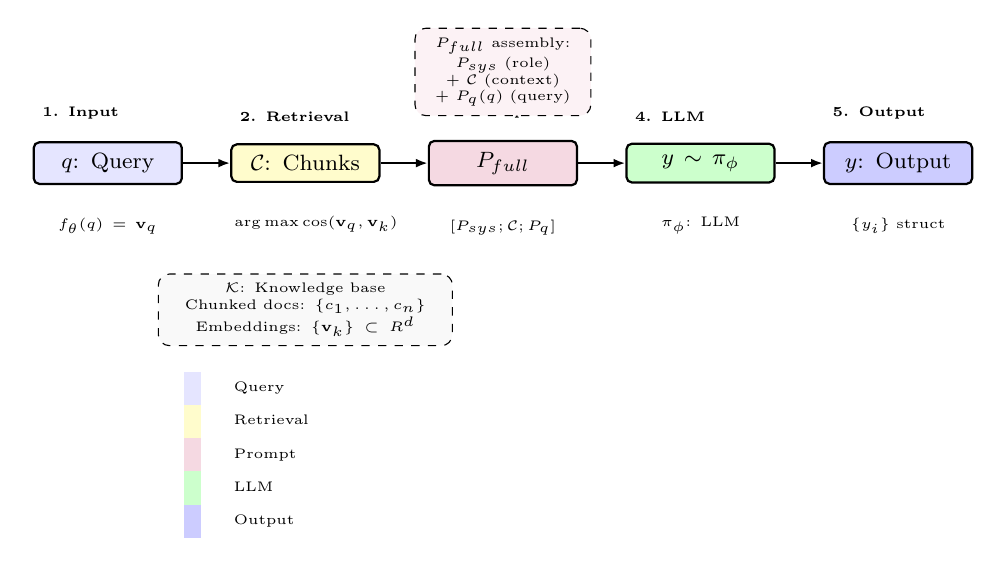
\begin{tikzpicture}[
  font=\footnotesize,
  block/.style={draw=black, rounded corners=2pt, thick, align=center, inner sep=4pt},
  arrow/.style={-{Latex[length=1.5mm]}, thick},
  formula/.style={font=\tiny, align=center, text width=1.8cm},
  node distance=0.8cm and 0.6cm
]

% ============================================================
% Main pipeline boxes (horizontal)
% ============================================================
\node[block, fill=blue!10, text width=1.6cm] (q) {$q$: Query};
\node[block, fill=yellow!20, text width=1.6cm, right=of q] (r) {$\mathcal{C}$: Chunks};
\node[block, fill=purple!15, text width=1.6cm, right=of r] (p) {$P_{\text{full}}$};
\node[block, fill=green!20, text width=1.6cm, right=of p] (l) {$y \sim \pi_\phi$};
\node[block, fill=blue!20, text width=1.6cm, right=of l] (o) {$y$: Output};

% Arrows
\draw[arrow] (q) -- (r);
\draw[arrow] (r) -- (p);
\draw[arrow] (p) -- (l);
\draw[arrow] (l) -- (o);

% ============================================================
% Stage labels above
% ============================================================
\node[font=\tiny\bfseries, above=0.15cm of q.north west, anchor=south west] {1. Input};
\node[font=\tiny\bfseries, above=0.15cm of r.north west, anchor=south west] {2. Retrieval};
\node[font=\tiny\bfseries, above=0.15cm of p.north west, anchor=south west] {3. Prompt};
\node[font=\tiny\bfseries, above=0.15cm of l.north west, anchor=south west] {4. LLM};
\node[font=\tiny\bfseries, above=0.15cm of o.north west, anchor=south west] {5. Output};

% ============================================================
% Formulas below each box
% ============================================================
\node[formula, below=0.3cm of q] (fq) {$f_\theta(q)=\mathbf{v}_q$};
\node[formula, below=0.3cm of r] (fr) {$\arg\max\cos(\mathbf{v}_q,\mathbf{v}_k)$};
\node[formula, below=0.3cm of p] (fp) {$[P_{\text{sys}};\mathcal{C};P_q]$};
\node[formula, below=0.3cm of l] (fl) {$\pi_\phi$: LLM};
\node[formula, below=0.3cm of o] (fo) {$\{y_i\}$ struct};

% ============================================================
% Knowledge base annotation (below retrieval formula)
% ============================================================
\node[draw=black, dashed, rounded corners, fill=gray!5, font=\tiny, below=0.4cm of fr, text width=3.5cm, align=center] (kb) {
$\mathcal{K}$: Knowledge base \\
Chunked docs: $\{c_1,\dots,c_n\}$ \\
Embeddings: $\{\mathbf{v}_k\}\subset\mathbb{R}^d$
};

% ============================================================
% Prompt composition detail (above prompt box)
% ============================================================
\node[draw=black, dashed, rounded corners, fill=purple!5, font=\tiny, above=0.3cm of p, text width=2cm, align=center] (pd) {
$P_{\text{full}}$ assembly: \\
$P_{\text{sys}}$ (role) \\
$+$ $\mathcal{C}$ (context) \\
$+$ $P_q(q)$ (query)
};

% ============================================================
% Legend (bottom left)
% ============================================================
\node[font=\tiny, anchor=north west, yshift=-0.2cm] at (kb.south west) {
\begin{tabular}{cl}
\colorbox{blue!10}{\strut} & Query \\
\colorbox{yellow!20}{\strut} & Retrieval \\
\colorbox{purple!15}{\strut} & Prompt \\
\colorbox{green!20}{\strut} & LLM \\
\colorbox{blue!20}{\strut} & Output
\end{tabular}};

\end{tikzpicture}

\caption{Pipeline architecture. The clinician query $q$ is embedded to $\mathbf{v}_q$, retrieves top-$k$ chunks $\mathcal{C}$ via cosine similarity from knowledge base $\mathcal{K}$, assembles full prompt $P_{\text{full}}$, and generates structured response $y$ via LLM $\pi_\phi$.}
\label{fig:model_architecture}
\end{figure}


% =====================FIGURE END==============================

\subsubsection{Response structure}

The LLM was constrained to generate responses following a structured format:
\begin{enumerate}
    \item \textbf{Where you are in the framework}: Identifies the current consultation phase
    \item \textbf{What needs to happen next}: Prioritized action items
    \item \textbf{Communication tools}: Sample language from toolkit
    \item \textbf{Stuck Points assessment}: Relational communication guidance when relevant
    \item \textbf{Suggested next step}: Single clear action
\end{enumerate}

This structure ensured consistent, actionable guidance while maintaining source fidelity.

\subsection{Evaluation Methodology}\label{sec:evaluation}

System evaluation addressed three dimensions: response quality, source grounding, and framework adherence.

\subsubsection{Quality assessment}

Response quality was evaluated by examining:
\begin{itemize}
    \item \textbf{Completeness}: Coverage of all required response sections
    \item \textbf{Clinical appropriateness}: Alignment with dementia care best practices
    \item \textbf{Language quality}: Clarity, conciseness, and actionability
\end{itemize}

\subsubsection{Source grounding evaluation}

Source fidelity was assessed by verifying that responses:
\begin{itemize}
    \item Drew directly from toolkit materials rather than external knowledge
    \item Correctly attributed guidance to appropriate framework components
    \item Declined to answer queries outside toolkit scope
\end{itemize}

The system was tested against a set of representative clinical scenarios covering each consultation phase and common stuck point situations.

\subsection{Ethical considerations}\label{sec:ethics}

This study involved the development and evaluation of an AI consultation assistant with clinician feedback sessions. The study was conducted under institutional guidelines for responsible AI development in healthcare.

The study did not involve patient data collection or processing. All content used for system development and evaluation was derived from publicly available clinical communication guidelines published by Ariadne Labs. No personally identifiable information was collected, stored, or processed during the development or evaluation phases.

\subsubsection{Risk, safety, and misuse considerations}

Foreseeable risks included over-reliance on model outputs, degraded performance on queries outside the toolkit scope, and potential for misleading guidance in sensitive clinical conversations. To mitigate these risks, the study was restricted to offline evaluation and did not expose the system to real patient consultations. The evaluation protocol explicitly tested the system's ability to decline out-of-scope queries, and failure cases were documented.

The system was designed with explicit source attribution requirements, reducing but not eliminating the risk of generating misleading guidance. Evaluation included verification that responses cited appropriate toolkit sources.

The system was tested with both frontier models (high-capability LLMs) and lighter models to identify an appropriate threshold balancing performance quality against computational efficiency. This approach prioritized practical deployability over maximal capability.

\subsubsection{Clinician feedback and human-AI interaction}

Clinicians provided feedback through a dual-mode evaluation interface that presented responses from multiple model providers simultaneously on identical inputs. This allowed direct comparison of model outputs and provided qualitative insights into clinical appropriateness.

Clinician feedback addressed:
\begin{itemize}
    \item \textbf{Relevance}: Whether guidance addressed the presented consultation scenario
    \item \textbf{Clinical tone}: Appropriateness of language for patient communication
    \item \textbf{Actionability}: Usefulness of suggested next steps and communication strategies
    \item \textbf{Safety}: Identification of potentially misleading or inappropriate suggestions
\end{itemize}

Feedback sessions informed iterative refinement of prompt templates and response structure. Clinicians noted that source attribution was essential for trust, and that responses declining out-of-scope queries were preferable to speculative guidance.

This feedback process constituted informal evaluation of human-AI interaction, though formal automation bias assessment was beyond scope. Future studies should explicitly measure decision override behavior and trust calibration.

\subsubsection{Equity and representational considerations}

This study evaluated an English-language consultation assistant using a clinical communication framework developed primarily for Western healthcare contexts. The Conversation Guides and Stuck Points Framework may not fully account for cultural variations in communication preferences, family involvement patterns, or healthcare system structures.

Clinician feedback was collected from a limited pool of English-speaking healthcare professionals. No demographic stratification was performed. Claims about system performance and appropriateness are limited to the evaluation scenarios tested and should not be generalized to all clinical populations or care settings.

\subsubsection{Carbon footprint and optimized computing resources}

The study used cloud-based LLM inference through provider APIs. API-based inference costs were tracked for budgeting purposes. No local model training was performed.

Model selection considered computational efficiency alongside performance, testing lighter alternatives to frontier models to identify practical deployment thresholds. The computational footprint was minimal compared to training approaches.

The study did not claim carbon neutrality. The primary environmental benefit was the use of pre-trained commercial models, which avoided training costs.

\subsubsection{Reproducibility and computational stewardship}

All evaluation prompts, scoring rubrics, and clinician feedback data were version-controlled in the project repository. Response generation used temperature-controlled API calls to ensure reproducibility of evaluation outputs. Model versions were documented to enable result reproduction.

Evaluation scenarios were defined prior to evaluation and stored as structured test cases, allowing repetition without regeneration of inputs.

Dual-mode evaluation outputs were logged and anonymized for reproducibility. The specific LLM providers and model versions tested were documented.

\subsubsection{Dual-use and downstream deployment considerations}

Although developed for clinical communication support, the methods could be adapted for other sensitive communication contexts beyond healthcare. This study avoids claims of deployment readiness and emphasizes that the system requires clinical validation, user interface refinement, and integration with clinical workflows before any clinical use.

The study explicitly documented failure modes, including the system's tendency to decline out-of-scope queries and quality boundaries of toolkit-grounded responses. These findings constrain claims about system utility.
